% !TeX spellcheck = en_GB
% %%% ***************** CHAPTER RESULTS ***************** %%%
\chapter{Results and Discussion} \label{ch:Res}
% \textcolor{red}{\textbf{The overleaf file from the Results is here:} \\ \url{https://www.overleaf.com/15070250fhqztvnygzmn}} 
% \\V
%
In this chapter the results of the surface observation, the optimal estimation retrieval and the regional mesoscale forecast model are presented. On the basis of the methodology described in \Cref{ch:Methods} it should be evaluated if a regional mesoscale forecast model predicts the same synoptic patterns as observed at the measurement site. Also, vertical SWC forecasted by MEPS is being compared with the retrieved vertical SWC at Haukeliseter. Attention should be paid to the fact, that this study study is unique. The motivation to compare regional model forecasts with vertical snowfall measurements resulted from a study by Joos and Wernli [2012]. They did sensitivity studies on the microphysical scheme of COSMO (COnsortium for Small-scale MOdelling) and found that the storm development depends on the correct vertical placement of the precipitation inside a modeled storm. Vertical precipitation determines the vertical profile of latent heating, and hence the generation of potential vorticity which in return shows if a storm strengthens or weakens. Correct vertical precipitation observations can then help to correctly assess model vertical precipitation patterns.

%As far as the author has knowledge of, no approach was done to verify a vertical regional forecast model with the help of vertical observation measurements. 
%%%%%%%%%%%%%%%%%%%%%%%%%%%%%%%%%%%%%%%%%%%%%%%%%%%%%%%%%%%%%%%%%%%%%%%%%%
\newpage
%%%%%%%%% retrieval sensitivity study %%%%%%%%%%%%%%
\section{Sensitivity of the optimal estimation retrieval}\label{sec:ret:sensitivity}
%%%%%%% image observed ice crystals %%%%%%%%%%%%%%%%
\begin{figure}[h]
	\centering
	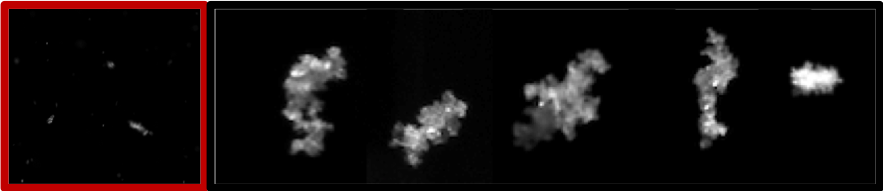
\includegraphics[width=0.8\textwidth]{./MASC_obs/blow_part}
	\caption{MASC observations during the Christmas storm 2016. Left (red frame), small ground up blowing snow particles. Five images on the right, rimed particles.}\label{fig:ret:all_part}
\end{figure}
%%%%%%%%%%%%%%%%%%%%%%%%%%%%%%%%%%%%%%%%%%%%%%
\noindent
The optimal estimation retrieval scheme was applied to the six-day Christmas 2016 storm event.  MASC images of snowfall during the event were used to guide the selection of the appropriate particle model and PSD input for the retrieval scheme. In this section, the sensitivity of retrieval results to these inputs is explored. Such an exercise should also allow an identification of those properties that yield the best match with Met Norway snow gauge measurements at Haukeliseter.  
\\
The majority of the MASC images from Haukeliseter contained snow particles that looked like the left image \Cref{fig:ret:all_part}. Such images suggest small ground-up blowing snow particles that are consistent with the high winds observed during the event.  However, a careful examination of the MASC images also finds the presence of rimed aggregates such as those in the right five images \Cref{fig:ret:all_part}. Pristine crystals such as plates and columns were not observed during this event.  As such, we explored the use of two different aggregate particle models developed for the CloudSat mission. 
\\
\Cref{fig:ret_sensitivity} presents hourly measured snowfall accumulations on \SI{22}{\dec} plotted against retrieved values for the two different aggregate assumptions. The 'B8' aggregate is a low reflectivity per unit mass aggregate that worked well for the cold, dry conditions observed at Barrow as described in \citet{cooper_variational_2017}.  The 'B6' aggregate is a high reflectivity per unit mass particle.  As such, the 'B6' aggregate would seem more physically consistent with the observed rimed particles and high water environment found in the coastal mountains at Haukeliseter.  The presence of a water or rimed coating on the aggregates aloft would greatly enhance their effective reflectivity. Indeed, \Cref{fig:ret_sensitivity} suggests that the reflective 'B6' aggregate agreed much better than the less reflective 'B8' aggregate with the snow gauge.
%
%Small ground up blowing snow particles (\Cref{fig:ret:all_part}, red frame), would follow the use of the CloudSat B8pr-30 particle model for the snowfall optimal estimation retrieval. This dry snow particle model was used at Barrow, Alaska \citep{cooper_variational_2017} and was for their study the best estimated result compared to National Weather Service station. Taking the same approach as \citet{cooper_variational_2017} and the assumption of small particles by the MASC would follow a too high estimates for surface snow accumulation (\Cref{fig:ret_sensitivity}). The temporal distribution of the snowfall during the event is shown in \Cref{fig:ret_sensitivity}. The figure presents hourly snowfall accumulations on \SI{22}{\dec} against retrieved values for different particle model assumptions. The CloudSat B8pr-30 particle model did not agree well in magnitude with the double fence hourly observations (blue, dash-dotted line). 
%The optimal estimation retrieval result for surface accumulation is too big, because the amount of mass needs to be high for small particles and much reflectivity would need to be generated. 
%%%%%%% image acc B6,B8 %%%%%%%%%%%%%%%%
\begin{figure}[t]
	\centering
	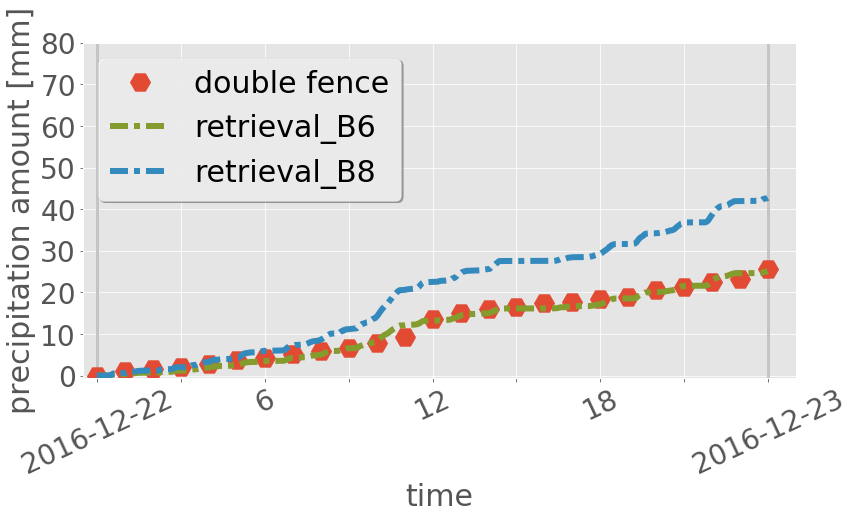
\includegraphics[width=0.8\textwidth]{./fig_obs_ret/20161222_2}
	\caption{Hourly double fence snowfall accumulations [mm] plotted against retrieved values for the \SI{22}{\dec} for different retrieval assumptions permutations. Double fence snowfall accumulation, red hexagons, retrieved precipitation amount for the here used study (B6), green, dash-dotted, and for small aggregates (B8), blue dashed.}\label{fig:ret_sensitivity}
\end{figure}
%%%%%%%%%%%%%%%%%%%%%%%%%%%%%%%%%%%%%%%%%%%%%%
%
\noindent
\\
%Since the surface snow accumulation for the most observed particles gives a too high amount, the optimal estimation retrieval is trained for rimed aggregates (\Cref{sec:ret_scheme}). These rimed particles were observed once in a while and the structure of the particles varied with wind directions. While small, round aggregates, furthest to the right in \Cref{fig:ret:all_part}, were more related to west wind, were the other four related to south-east wind.
%%%%%%% table error sfc acc ret sensitivity %%%%%%%%%%%%%%%%
\begin{table}[t]
	\begin{center}
		\caption{Observations (obs.) and retrieved (ret.) snowfall amounts for \SI{22}{\dec} for different particle model assumptions. B6 indicating the here uses particle model (\Cref{app:scat_scheme}) and B8 indicating the retrieved snowfall amounts for small particles.}\label{tab:res:ret_sens}
		\begin{tabular}{c||r|r|c||r|r|c}
			\hline \hline
			& \multicolumn{3}{c||}{\textbf{\SI{12}{\hour} accumulation}} & \multicolumn{3}{c}{\textbf{\SI{24}{\hour} accumulation}}    \\\cline{2-7}
			\textbf{Particle} & \multicolumn{2}{c|}{\textbf{Snowfall}} & \textbf{Difference} &  \multicolumn{2}{c|}{\textbf{Snowfall}} & \textbf{Difference}   \\\cline{2-3} \cline{5-6}
			\textbf{model} & \textbf{obs.} & \textbf{ret.} && \textbf{obs.} & \textbf{ret.} &  \\\cline{2-7}
			& \multicolumn{2}{c|}{[\SI{}{\mm}]} & [\SI{}{\percent}]  & \multicolumn{2}{c|}{[\SI{}{\mm}]} & [\SI{}{\percent}]  \\ \hline\hline
			B6  & \num{13.6} &\num{13.2} & \num{-3.0} & \num{23.1} & \num{25.1} & \num{- 2.1}  \\\hline
			B8  & \num{13.6} &\num{22.5} & +\num{65.5} & \num{23.1} & \num{42.7} & +\num{66.9}  \\\hline\hline
		\end{tabular}
	\end{center}
\end{table}

%%%%%%%%%%%%%%%%%%%%%%%%%%%%%%%%%%%%%%%%%%%%%%%%%%%%%%%%%%%%%%%%%%%%%%%%%%
%
\noindent
%The best guess were found for the 2D-scattering model for branched 6-arm spatial particles with porosity for reflectivity measurements at \SI{24}{\giga\hertz} (B6, \Cref{app:scat_scheme}). This scattering scheme relates to the five crystals to the right in \Cref{fig:ret:all_part}. The percentage difference was small compared to the double fence observations throughout the event (\Cref{tab:res:ret_error}) for \SIlist{12;24}{\hour} surface accumulation.
\\
%\Cref{tab:res:ret_sens} presents the percentage differences for both particle model assumptions, on \SI{22}{\dec}. The percentage difference for \SI{12}{\hour} surface accumulation indicated an overestimation of \SI{65}{\percent} for very small, blowing like particles.
\Cref{tab:res:ret_sens} presents the percentage differences between snow gauge and retrieved estimates found when using these particle model assumptions for \SI{22}{\dec}. Use of the 'B6' aggregate agreed within \SI{5}{\percent} of the double fence observations (\Cref{tab:res:ret_sens}) for both \SI{12}{\hour} and \SI{24}{\hour} surface accumulations. Admittedly, use of the ‘B6’ aggregate produced slightly too little snowfall relative to the gauges for the remaining days of the event as discussed in \Cref{sec:ret_dofe_comp}. The use of the ‘B8’ aggregate, however, overestimated snowfall by at least \SI{65}{\percent} for both the \SI{12}{\hour} and \SI{24}{\hour} surface accumulations (\Cref{tab:res:ret_sens}). Since this aggregate had low reflectivity per unit mass, it required significantly more SWC in the forward model calculations to match MRR reflectivities. The retrieval therefore overestimates snowfall rate for these meteorological conditions.
%\\
%The rimed particle model produced slightly too little snowfall for most of the days throughout the event (\Cref{tab:res:ret_error}). Values for \SI{22}{\dec} showed to have the best agreement for \SIlist{12;24}{\hour} (\SIlist{-3.0;-2.1}{\percent}).
%\\
%It shows, when very turbulent storms prevail, the approach does not work like for more intense, humid storms, because the particles are too small and the assumption of blowing, small particles give an overestimation at the ground. 
%It follows from the good agreement between the retrieved surface snowfall amount and the double fence observations with the use of the rimed particle model assumption, that it is important to know what kind of particles are in the storm to get the correct aggregate for the a priori guess in the optimal estimation retrieval. MASC observations would assume to use the CloudSat B8pr-30 particle model, but that would not give the correct answer (\Cref{fig:ret_sensitivity} and \Cref{tab:res:ret_sens}). The use of MRR reflectivity and MASC habit can lead to a closer answer compared to double fence measurements.
\\
The discussion here has focused on MASC estimates of habit instead of PSD or fall speed. The reason is that the MASC and PIP saw primarily blowing snow particles at the surface that likely were much smaller than the particles that the MRR remotely sensed aloft.  The use of the PSD measured by the MASC or PIP in the retrieval therefore produced snowfall totals much greater than those measured by the double fence snow gauges.  Essentially, it takes a much greater mass of small particles than large particles to match a given reflectivity. These results contrast with those found for low wind speed events at Haukeliseter where the use of MASC habit, PSD, and fall speed observations resulted in retrieved snowfall accumulations very close to Met Norway snow gauge observations.  Regardless, for this high wind event, the \citet{wood_estimation_2011} a priori temperature PSD relationship and a climatological average fallspeed of \SI{0.85}{\mPs} \citep[private communication,][]{Priv_Comm_Schirle} were employed.




%%%%%%%%% Observation agreement %%%%%%%%%%%%%%
\section{Comparison of surface observations} \label{sec:ret_dofe_comp}
To be able to compare the vertical predicted snow water content with the retrieved snow water content a verification of the surface accumulation is made. If the retrieved surface accumulation is confident in comparison to the double fence measurement, then the vertical measurements can be trusted.
\\
The correlation in \Cref{fig:res:obs_ret_scatter} demonstrates a good agreement between the \SI{48}{\hour} accumulation measured by the double fence and the retrieved surface accumulation.
The black line in \Cref{fig:res:obs_ret_scatter} presents a linear correlation with a regression coefficient of R = \num{0.97}. 
In general, the retrieved surface snowfall accumulation is underestimated when compared to the double fence measurements, but not to a large degree. 
\\
\Cref{fig:res:diff_ret_scatter} shows the difference between retrieved accumulation and observed accumulation by the double fence. For the time period \num{20} to \SI{24}{\dec}, \Cref{fig:res:diff_ret_scatter} indicates an underestimation of retrieved snow accumulation of less than \SI{-5}{\mm} for the first \SI{24}{\hour}. 
Snow accumulation calculated on \SI{23}{\dec} at \SI{0}{\UTC} show after \SI{24}{\hour} an underestimation by the retrieval of up to \SI{-6.5}{\mm}. Larger underestimation after \SI{43}{\hour} is related to the observation of liquid precipitation on \SI{25}{\dec} between \SIrange{12}{21}{\UTC} for accumulations on \SI{24}{\dec}. On \SI{25}{\dec} no fair comparison to the double fence measurement can be performed after \SI{12}{\UTC} because of the neglection of liquid precipitation when temperatures exceed \SI{2}{\celsius}.
\\
%The mean absolute difference of all days is \SI{2.06}{\mm} (excluding values on \SI{25}{\dec} after \SI{12}{\UTC} and on \SI{26}{\dec} after \SI{17}{\UTC} because of attenuation at the MRR). 
For a \SI{12}{\hour} accumulation follows for the Christmas storm (\num{20} to \SI{26}{\dec}) an average error of \SI{85.5}{\percent} (\Cref{tab:res:ret_error}). For longer, \SI{24}{\hour} accumulation decreases the average error to be \SI{- 4.7}{\percent} (excluding values on \SI{25}{\dec} after \SI{12}{\UTC} and on \SI{26}{\dec} after \SI{17}{\UTC} because of attenuation at the MRR). The daily surface snowfall accumulation difference between retrieval and observation in \Cref{tab:res:ret_error} show almost always a well agreement to the boundary condition of the double fence. The only well pronounced mismatch is seen non \SI{21}{\dec}, where it measures much more than the double fence gauge (+\SI{435.8}{\percent}).
%%%%%%% image scatter obs ret %%%%%%%%%%%%%%%%
\begin{figure}[t]
	\centering
	\begin{subfigure}[b]{0.38\textwidth}
		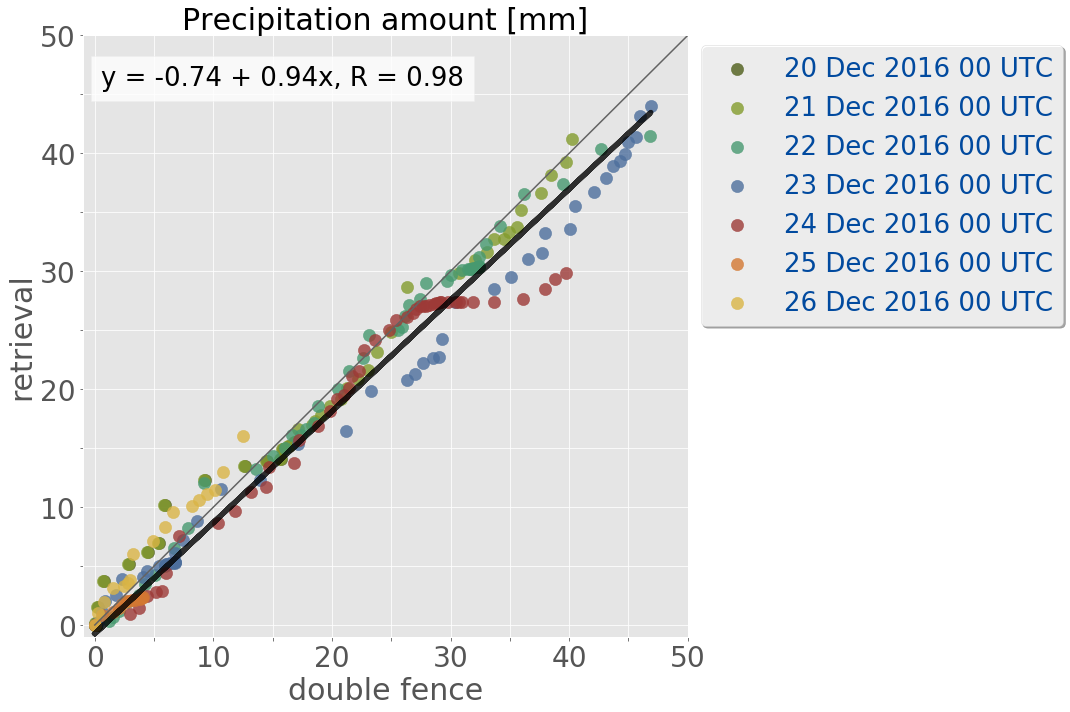
\includegraphics[trim={0.cm 0.cm 13cm 0cm},clip,
		width=\textwidth]{./fig_obs_ret/obs_ret_20161220_26_00}
		\caption{}\label{fig:res:obs_ret_scatter}
	\end{subfigure}
	%
	\begin{subfigure}[b]{0.59\textwidth}
		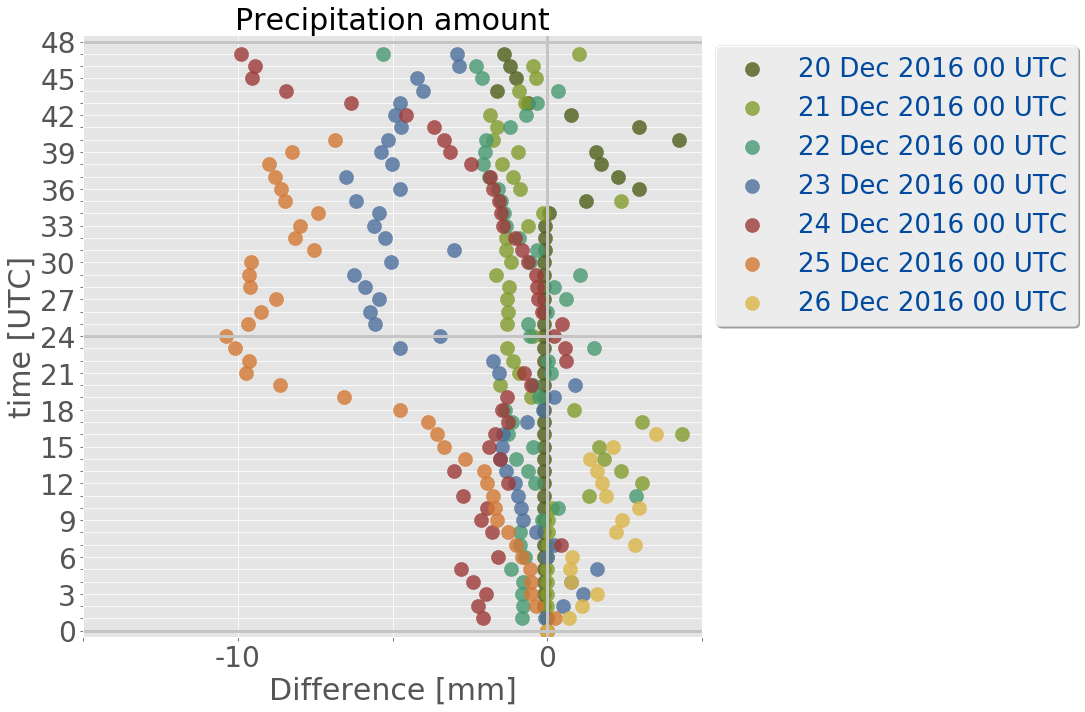
\includegraphics[trim={0.cm 0.cm 0cm 0cm},clip,
		width=\textwidth]{./fig_obs_ret/diff_20161220_26_00}
		\caption{}\label{fig:res:diff_ret_scatter}
	\end{subfigure}
	% label
	%    \begin{subfigure}[t]{0.18\textwidth}
	%   	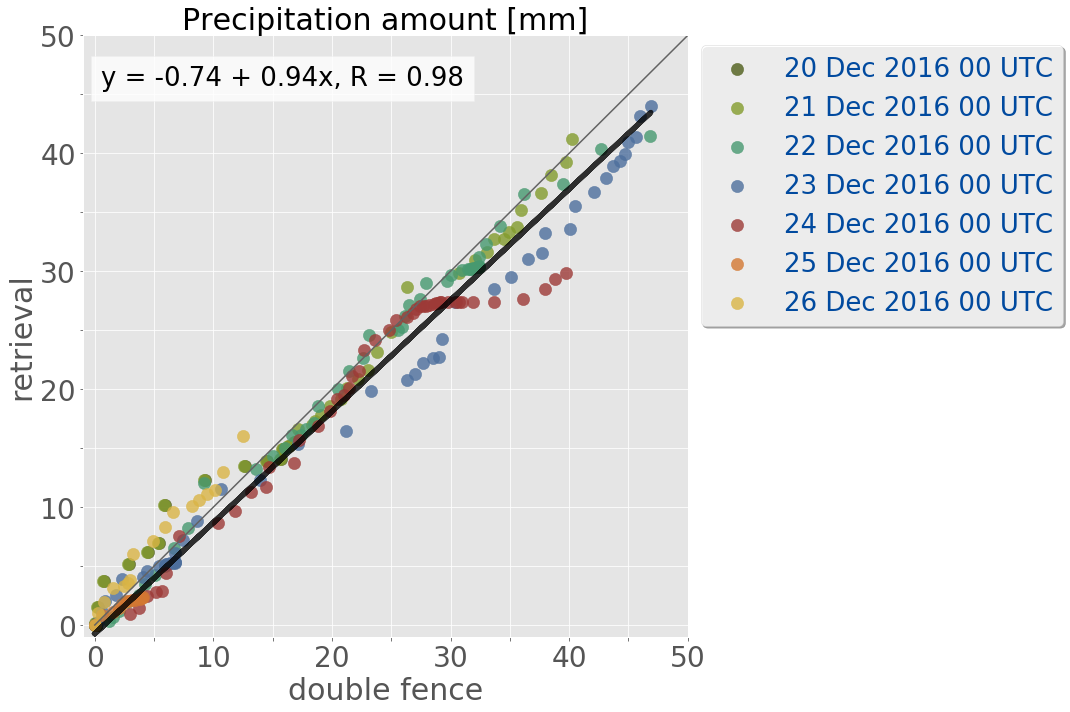
\includegraphics[trim={25.cm 13.cm 0cm 1.3cm},clip,
	%  width=\textwidth]{./fig_obs_ret/obs_ret_20161220_26_00}
	% \end{subfigure}
	\caption{\protect\subref{fig:res:obs_ret_scatter}: Surface precipitation amount comparison between the double fence observations and the retrieved surface accumulation of precipitation for \SI{48}{\hour}. In black the linear correlation between the double fence observations and retrieved surface snow. 
		\protect\subref{fig:res:diff_ret_scatter}: Difference between the retrieved and the observed accumulation by the double fence. The colours represent the different starting days at \SI{0}{\UTC} for the \SI{48}{\hour} accumulation.}\label{fig:res:obs_ret}
\end{figure}
%%%%%%%%%%%%%%%%%%%%%%%%%%%%%%%%%%%%%%%%%%%%%%
\\
Similar to this study, \citet{cooper_variational_2017} used a CloudSat snow particle model, PSD and fall speed from MASC observations for five snow events at Barrow, Alaska. The comparison to the weather station revealed an difference between National Weather Service observations and retrieved accumulations of \SI{- 18}{\percent} for all five snow events.
%%%%%%% table error sfc acc ret obs %%%%%%%%%%%%%%%%
\begin{table}[t!]
	\begin{center}
		\caption{Comparison of observed (obs.) and retrieved (ret.) snowfall amounts for the Christmas storm 2016. Difference refers to the difference of the retrieved and observed snow accumulation after \SI{12}{\hour} and \SI{24}{\hour}. The average difference is the value over all six/four days. Excluding values after \SI{12}{\UTC} on \SI{25}{\dec} and after \SI{17}{\UTC} on \SI{26}{\dec}.}\label{tab:res:ret_error}
		\begin{tabular}{c||r|r|c|c||r|r|c|c}
			\hline \hline
			& \multicolumn{4}{c||}{\textbf{\SI{12}{\hour} accumulation}} & \multicolumn{4}{c}{\textbf{\SI{24}{\hour} accumulation}}    \\ \cline{2-9}
			\textbf{Day} & \multicolumn{2}{c|}{\textbf{Snowfall}} & \textbf{Difference} & \textbf{Average} &  \multicolumn{2}{c|}{\textbf{Snowfall}} & \textbf{Difference} & \textbf{Average}  \\\cline{2-3} \cline{6-7}
			\textbf{in 2016} & \textbf{obs.} & \textbf{ret.} & & \textbf{difference} & \textbf{obs.} & \textbf{ret.} & & \textbf{difference} \\\cline{2-9}
			& \multicolumn{2}{c|}{[\SI{}{\mm}]} & [\SI{}{\percent}] & [\SI{}{\percent}] & \multicolumn{2}{c|}{[\SI{}{\mm}]} & [\SI{}{\percent}] & [\SI{}{\percent}] \\ \hline\hline
			\num{20} Dec & \num{0.1} &\num{0.0} & \num{-97.8} & & \num{0.1} & \num{0.0} & \num{- 97.8} &  \\\cline{1-9}
			\num{21} Dec & \num{0.7} & \num{3.8} & +\num{435.8} & \multirow{6}{*}{+\num{85.5}} & \num{17.1} & \num{16.6} & \num{-2.7} & \multirow{4}{*}{\num{-4.7}}   \\\cline{1-4}\cline{6-8}
			\num{22} Dec & \num{13.6}& \num{13.2} & \num{- 3.0} & & \num{25.6} &\num{25.1} & \num{-2.1} &   \\\cline{1-4}\cline{6-8}
			\num{23} Dec & \num{6.3} &\num{5.2} & \num{- 16.8} & & \num{23.3}& \num{19.8} & \num{-14.9} &   \\\cline{1-4}\cline{6-8}
			\num{24} Dec & \num{14.7} & \num{13.4} & \num{- 8.6} && \num{24.8} & \num{25.0} & +\num{0.8} &   \\\cline{1-4}\cline{6-9}
			\num{25} Dec &  \num{4.3} & -- & -- & & +\num{15.4} & -- & -- & \\\cline{1-4}\cline{6-9}
			\num{26} Dec & \num{8.8} & \num{10.6} & +\num{20.1} &  &  \num{25.1} &-- & -- &  \\\hline\hline
		\end{tabular}
	\end{center}
\end{table}
%%%%%%%%%%%%%%%%%%%%%%%%%%%%%%%%%%%%%%%%%%%%%%
\\
\Cref{tab:res:ret_error} shows the difference for each individual day and the average difference for six and 4 days, depending on the accumulation of \SI{12}{\hour} or \SI{24}{\hour}.
The choice of the correct PSD model, slope parameters and fall speed in the optimal estimation snowfall retrieval, shows a good agreement with the observations at Haukeliseter for the 2016 Christmas storm in contrast to the \SI{200}{\percent} difference when only using the CloudSat snowfall algorithm \Cref{sec:retrieval}. It indicates also that the non-uniqueness of snow accumulation is reduced, when using a combination of ground-based observations instead of only Ze-S relationships. 
%Of course, more storms should be investigated to find the exact correlation between the surface observations and the estimated accumulation to see if the deviation keeps as small for different snow patterns at Haukeliseter. 
During the 2016 Christmas storm the average error for \SI{24}{\hour} accumulation is almost similar to the best estimate at Barrow, Alaska. It turns out that there is no relation between high and low precipitation events since the differences vary. \citet{cooper_variational_2017} also showed different combinations of PSD assumptions and snow fall speed. For Barrow, best agreements between observations and retrieved snowfall were found by using the CloudSat particle model, slope parameters and snowfall speeds from the MASC. In the here presented study, the best assumption for surface snowfall accumulation was found by using a particle model for rimed aggregates (\Cref{sec:retrieval} and \ref{sec:ret:sensitivity}) such as in \Cref{fig:ret:all_part}. 
\\
\\
On \num{20} and \SI{21}{\dec}, the difference error is large (\SI{-97.8}{\percent} and \SI{435.8}{\percent}, respectively). This is probably related to an observation of precipitation at the double fence, even though no precipitation was observed. The double fence observation might be related to some particles stirred up by wind into the orifice of the gauge. Since no manual observations are done at the Haukeliseter site, is it difficult to say if blowing snow occurred and might introduce additional errors. But from the vertical MRR reflectivity it can be seen, that precipitation was not observed on before \SI{21}{\dec} \SI{9}{\UTC}.
\\
Even though it is assumed that the double fence is the absolute correct measurement it still underlies some uncertainties. 
A better way to asses the accuracy of the retrieved surface snowfall accumulation could be to compare the results to measurements inside a bush gage. A bush gauge is a precipitation gauge surrounded by a large bush to create artificial calm winds to increase the catch ratio of frozen precipitation and is considered as the best available measurement for solid precipitation \citep{wolff_wmo_2018}. Unfortunately there are only two bush gauges in the world, and because of local limitations a double fence construction is developed as reference for the Solid Precipitation Measurement intercomparison study during \numrange{1986}{1993} \citep{goodison_wmo_1998}. Comparisons between bush gauge and double fence precipitation measurements have shown, that for wind speeds up to \SI{9}{\mPs} outside the fence, the double fence will measure up to \SI{10}{\percent} less precipitation. 
While wind speeds outside the double fence might reach \SI{20}{\mPs} show measurements inside a decrease to \SI{5}{\mPs}. \citet{wolff_wmo_2018} believes the underestimation of the double fence will not be more than \SI{20}{\percent} during frozen precipitation events with high wind speeds. 
\\
The low average difference value for \SI{24}{\hour} accumulation, in \Cref{tab:res:ret_error} during the Christmas 2016 event (\SI{-4.7}{\percent}) follows a much lower average difference between retrieved and observed surface accumulation than at Barrow (\SI{36}{\percent}) and therefore a very good agreement between observed and retrieved snow accumulation during \num{21} to \SI{24}{\dec}. In \Cref{sec:res:verticalSWC}, the vertical SWC will be compared to the forecasted MEPS values for the 2016 Christmas storm. Despite the condition that the double fence measurement is influenced by wind will the small average difference for \num{21} to \SI{24}{\dec} give confidence in the retrieved profiles of snow water content when comparing to the forecast, but it should be kept in mind that retrieved snow accumulation is underestimated and therefore may the vertical SWC be too low.
%%%%%%%%%%%%%%%%%%%%%%%%%%%%%%%%%%%%%%%%%%%%%%%%%%%%%%%%%%%%%%%%%%%%%%%%%%




